%!TEX program = xelatex
\documentclass[12pt]{article}

\usepackage[english]{babel}
\usepackage{xeCJK}

% Set page size and margins
\usepackage[a4paper,top=2cm,bottom=2cm,left=3cm,right=3cm,marginparwidth=1.75cm]{geometry}

% Useful packages
\usepackage{amsmath}
\usepackage{graphicx}
\graphicspath{{figure/}{figures/}{實驗結報二/figure/}{../實驗結報一/figure/}{實驗結報一/figure/}}
\usepackage[colorlinks=true, allcolors=blue]{hyperref}

\usepackage{array}
\newcolumntype{P}[1]{>{\centering\arraybackslash}p{#1}}
\newcolumntype{M}[1]{>{\centering\arraybackslash}m{#1}}

\usepackage{adjustbox}
\usepackage{caption}
\usepackage{subcaption}
\usepackage{siunitx}
\usepackage{float}

% ----- paragraph -----
\usepackage{titlesec}
\setcounter{secnumdepth}{4}
\titleformat{\paragraph}
{\normalfont\normalsize\bfseries}{\theparagraph}{1em}{}
\titlespacing*{\paragraph}
{0pt}{3.25ex plus 1ex minus .2ex}{1.5ex plus .2ex}
% ----- paragraph ----

% Prefer your original font, then use safe fallbacks available in common setups.
\IfFontExistsTF{NotoSerifTC-Regular}{
  \setCJKmainfont{NotoSerifTC-Regular}[AutoFakeBold = 3]
  \setCJKsansfont{NotoSerifTC-Regular}[AutoFakeBold = 3]
  \setCJKmonofont{NotoSerifTC-Regular}[AutoFakeBold = 3]
}{
  \IfFontExistsTF{Noto Serif CJK TC}{
    \setCJKmainfont{Noto Serif CJK TC}
    \setCJKsansfont{Noto Serif CJK TC}
    \setCJKmonofont{Noto Serif CJK TC}
  }{
    \IfFontExistsTF{Songti TC}{
      \setCJKmainfont{Songti TC}
      \setCJKsansfont{Songti TC}
      \setCJKmonofont{Songti TC}
    }{
      \setCJKmainfont{FandolSong-Regular}
      \setCJKsansfont{FandolSong-Regular}
      \setCJKmonofont{FandolFang-Regular}
    }
  }
}

\usepackage{indentfirst}
\setlength\parindent{24pt}

\begin{document}

\begin{titlepage}
  \begin{center}
      \vspace*{1cm}
       \begin{LARGE} 
           \textbf{
           \\ 數位電路實驗結報三
           \\ \
           \\ -- 平衡車 --
           }
       \end{LARGE}
      \vspace{0.5cm}
        \textbf{}
          
      \vspace{1.5cm}

      \textbf{Group 2: B11303052 蘇盈翰 (Right), B11702091 張容爾 (Middle), B10901144 王俊皓 (Left)}
       
      \vspace{1.5cm}

      \text{\today}

      \vspace{0.8cm}

      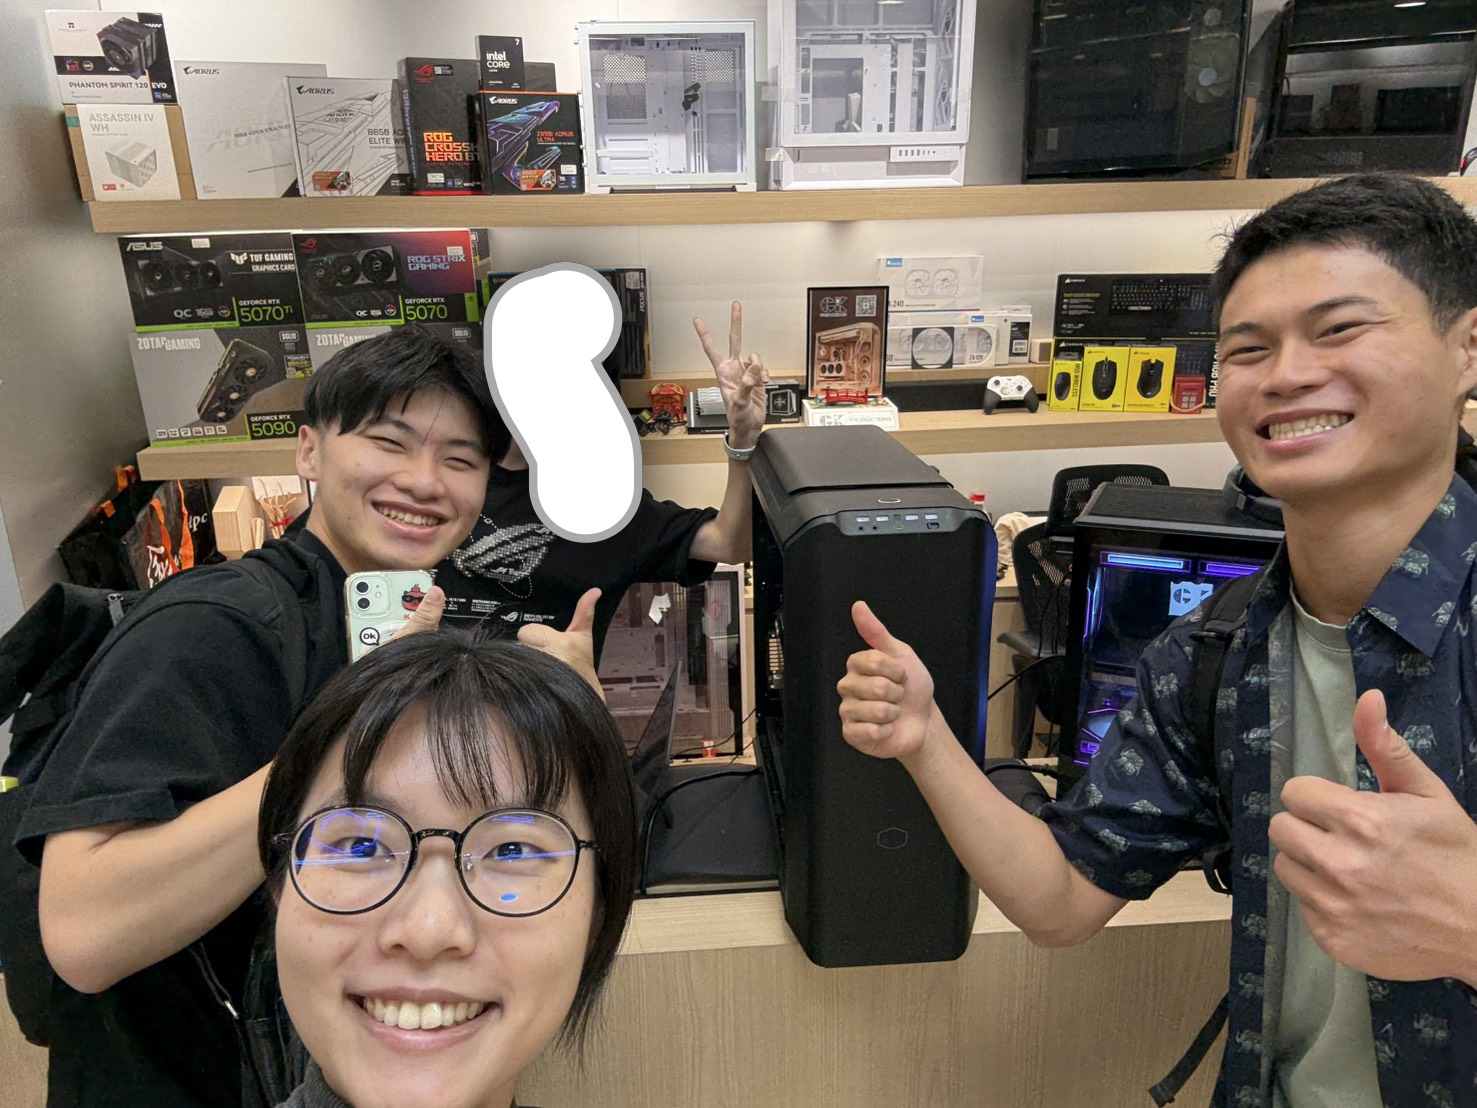
\includegraphics[width=0.7\textwidth]{Member.jpg}
     
      \vfill
          
      \vspace{0.8cm}
     
  \end{center}
\end{titlepage}

\section{實驗原理}

\subsection{電路板（PCB）焊接}

傳統麵包板接線容易因接觸不良造成電路不穩定，且佔用空間龐大；電路板（PCB）焊接則可省略複雜的接線過程、縮小電路體積、提升穩定性，同時便於量產。本次實驗使用預先以 EasyEDA 軟體設計的客製化電路板，再焊接上各功能模組，達成平衡車所需之電路整合。

焊接的目標是在接點上形成金字塔型銲錫包覆。良好的焊接接點應具備：錫量適中（金字塔狀）、充分受熱（光亮圓潤）、無虛焊（cold joint）。常見的焊接缺陷包括錫量過多（球狀）、錫量不足（平坦）、冷焊（暗沉粗糙）以及短路（solder bridge，相鄰腳位被錫橋接）。

\subsection{平衡車電路架構}

本實驗之平衡車控制電路包含以下核心元件：

\begin{itemize}
    \item \textbf{ESP32（NodeMCU-32S）}：主控制器，負責讀取感測器數據、執行 PID 演算法並輸出馬達控制訊號，同時建立 Wi-Fi 存取點供手機端連線調整參數。
    \item \textbf{MPU-6050}：六軸慣性測量單元（IMU），整合三軸陀螺儀與三軸加速度計，透過 I$^2$C 介面（SCL、SDA）與 ESP32 通訊，提供車體傾斜角度數據。
    \item \textbf{A4988 $\times$ 2}：步進馬達驅動 IC，接受 ESP32 發出之 STEP 與 DIR 訊號，分別驅動左右兩顆步進馬達，支援微步進控制（MS1--MS3）。
    \item \textbf{LM2596 降壓模組}：將電池電壓（約 12\,V）降壓至穩定之 5\,V，供 ESP32 與感測器使用，並以開關（SW1）控制整體電源通斷。
    \item \textbf{100\,\si{\micro\farad} 濾波電容 $\times$ 2}：穩定電源線電壓，減少步進馬達運轉時產生的電源雜訊對控制邏輯的干擾。
\end{itemize}

\subsection{PID 自動控制原理}

\subsubsection{回饋控制系統}

PID 控制器屬於閉迴路回饋控制（Closed-loop Feedback Control）。其基本運作方式為：感測器持續量測受控系統（Plant）的輸出值 $y(t)$，計算與目標值 $r(t)$ 之間的誤差 $e(t) = r(t) - y(t)$，再依據 PID 三個項目的加權和決定控制輸出 $u(t)$，驅動系統修正誤差。

簡單的開關控制（on/off controller）可將參數維持在目標範圍內，但系統會持續在目標值附近震盪而無法到達穩態。PID 控制器透過連續可調的回饋訊號，能夠消除穩態誤差並抑制震盪，同時縮短收斂時間。

\subsubsection{P、I、D 三項}

PID 控制器之輸出 $u(t)$ 定義為：

\begin{equation}
    u(t) = K_p \, e(t) \;+\; K_i \int_0^t e(\tau)\,d\tau \;+\; K_d \,\frac{de(t)}{dt}
\end{equation}

\begin{itemize}
    \item \textbf{比例項 $K_p$（Proportional）}：根據當前誤差的大小成比例地輸出控制量。$K_p$ 越大，系統響應越快，但過大則易導致超調（overshoot）與震盪不穩。
    \item \textbf{積分項 $K_i$（Integral）}：對誤差隨時間的累積積分進行補償，能夠消除穩態誤差（steady-state error）。$K_i$ 過大會增加超調量並延長收斂時間（settling time）。
    \item \textbf{微分項 $K_d$（Derivative）}：根據誤差的變化率（微分）預測趨勢並提前反應，能有效降低超調與縮短震盪衰減時間。$K_d$ 過大則易放大感測器雜訊。
\end{itemize}

各參數對系統行為的影響整理如表~\ref{tab:pid_effects}。

\begin{table}[H]
    \centering
    \begin{tabular}{lllll}
        \hline
        \textbf{參數增大} & \textbf{Rise time} & \textbf{Overshoot} & \textbf{Settling time} & \textbf{Steady-state error} \\
        \hline
        $K_p$ & Decrease & Increase & Small change & Decrease \\
        $K_i$ & Decrease & Increase & Increase     & Eliminate \\
        $K_d$ & Minor change & Decrease & Decrease  & No effect \\
        \hline
    \end{tabular}
    \caption{PID 三個參數對系統響應的影響}
    \label{tab:pid_effects}
\end{table}

對平衡車而言，目標值 $r(t) = 0$（直立，傾斜角為零），感測量 $y(t)$ 為 MPU-6050 回報之車體傾斜角，控制輸出 $u(t)$ 則映射為兩顆步進馬達的轉速與方向，以抵消車體傾倒趨勢。


\section{實驗架設與步驟}

\subsection{Week 9：電路板焊接}

\subsubsection{元件清單}

每人一份：PCB 電路板一片、開關（SW1）、排針母座、2P 端子台、100\,\si{\micro\farad} 電容 $\times$ 2。一組一份：ESP32 模組、MPU-6050 模組、A4988 步進馬達驅動模組 $\times$ 2、LM2596 降壓模組。

\subsubsection{焊接步驟}

\begin{enumerate}
    \item 將海綿沾濕但不滴水，將溫控烙鐵放置於烙鐵架上並清空周圍物品。
    \item 插上電源，調整溫度至 300\,°C 以上，待溫度穩定後開始焊接。
    \item 將元件（開關、排針母座、端子台、電容）插入電路板孔位，平貼底部並以膠帶固定後翻至背面。
    \item 一手拿錫線，一手持烙鐵，先加熱元件腳位與電路板焊墊（pad）約 2--3 秒，再將錫線推向烙鐵前端；錫融化後會自然堆積於接點形成金字塔狀。
    \item 移開烙鐵，待銲點自然冷卻，目視確認銲點光亮飽滿、無虛焊或短路。
    \item 使用斜口鉗剪去電路板背面多餘的元件腳位。每焊接數個接點後以濕海綿清潔烙鐵頭。
\end{enumerate}

\subsubsection{電路板測試}

焊接完成後，以三用電表導通模式（蜂鳴器模式）逐一確認各模組的電源（VCC）與接地（GND）焊接點是否正確導通，確認範圍包含：LM2596 模組輸出端、MPU-6050 電源腳位、兩個 A4988 模組電源腳位以及 ESP32 電源腳位。確認無誤後請助教進行最終檢查。

本組電路板正面（插件元件）與背面（焊點）如圖~\ref{fig:pcb_soldered} 所示。

\begin{figure}[H]
    \centering
    \begin{subfigure}[t]{0.45\textwidth}
        \centering
        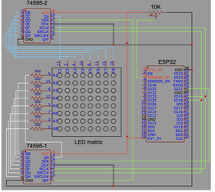
\includegraphics[width=\textwidth]{circuit_logic.png}
        \caption{平衡車電路邏輯圖}
        \label{fig:pcb_logic}
    \end{subfigure}
    \hfill
    \begin{subfigure}[t]{0.45\textwidth}
        \centering
        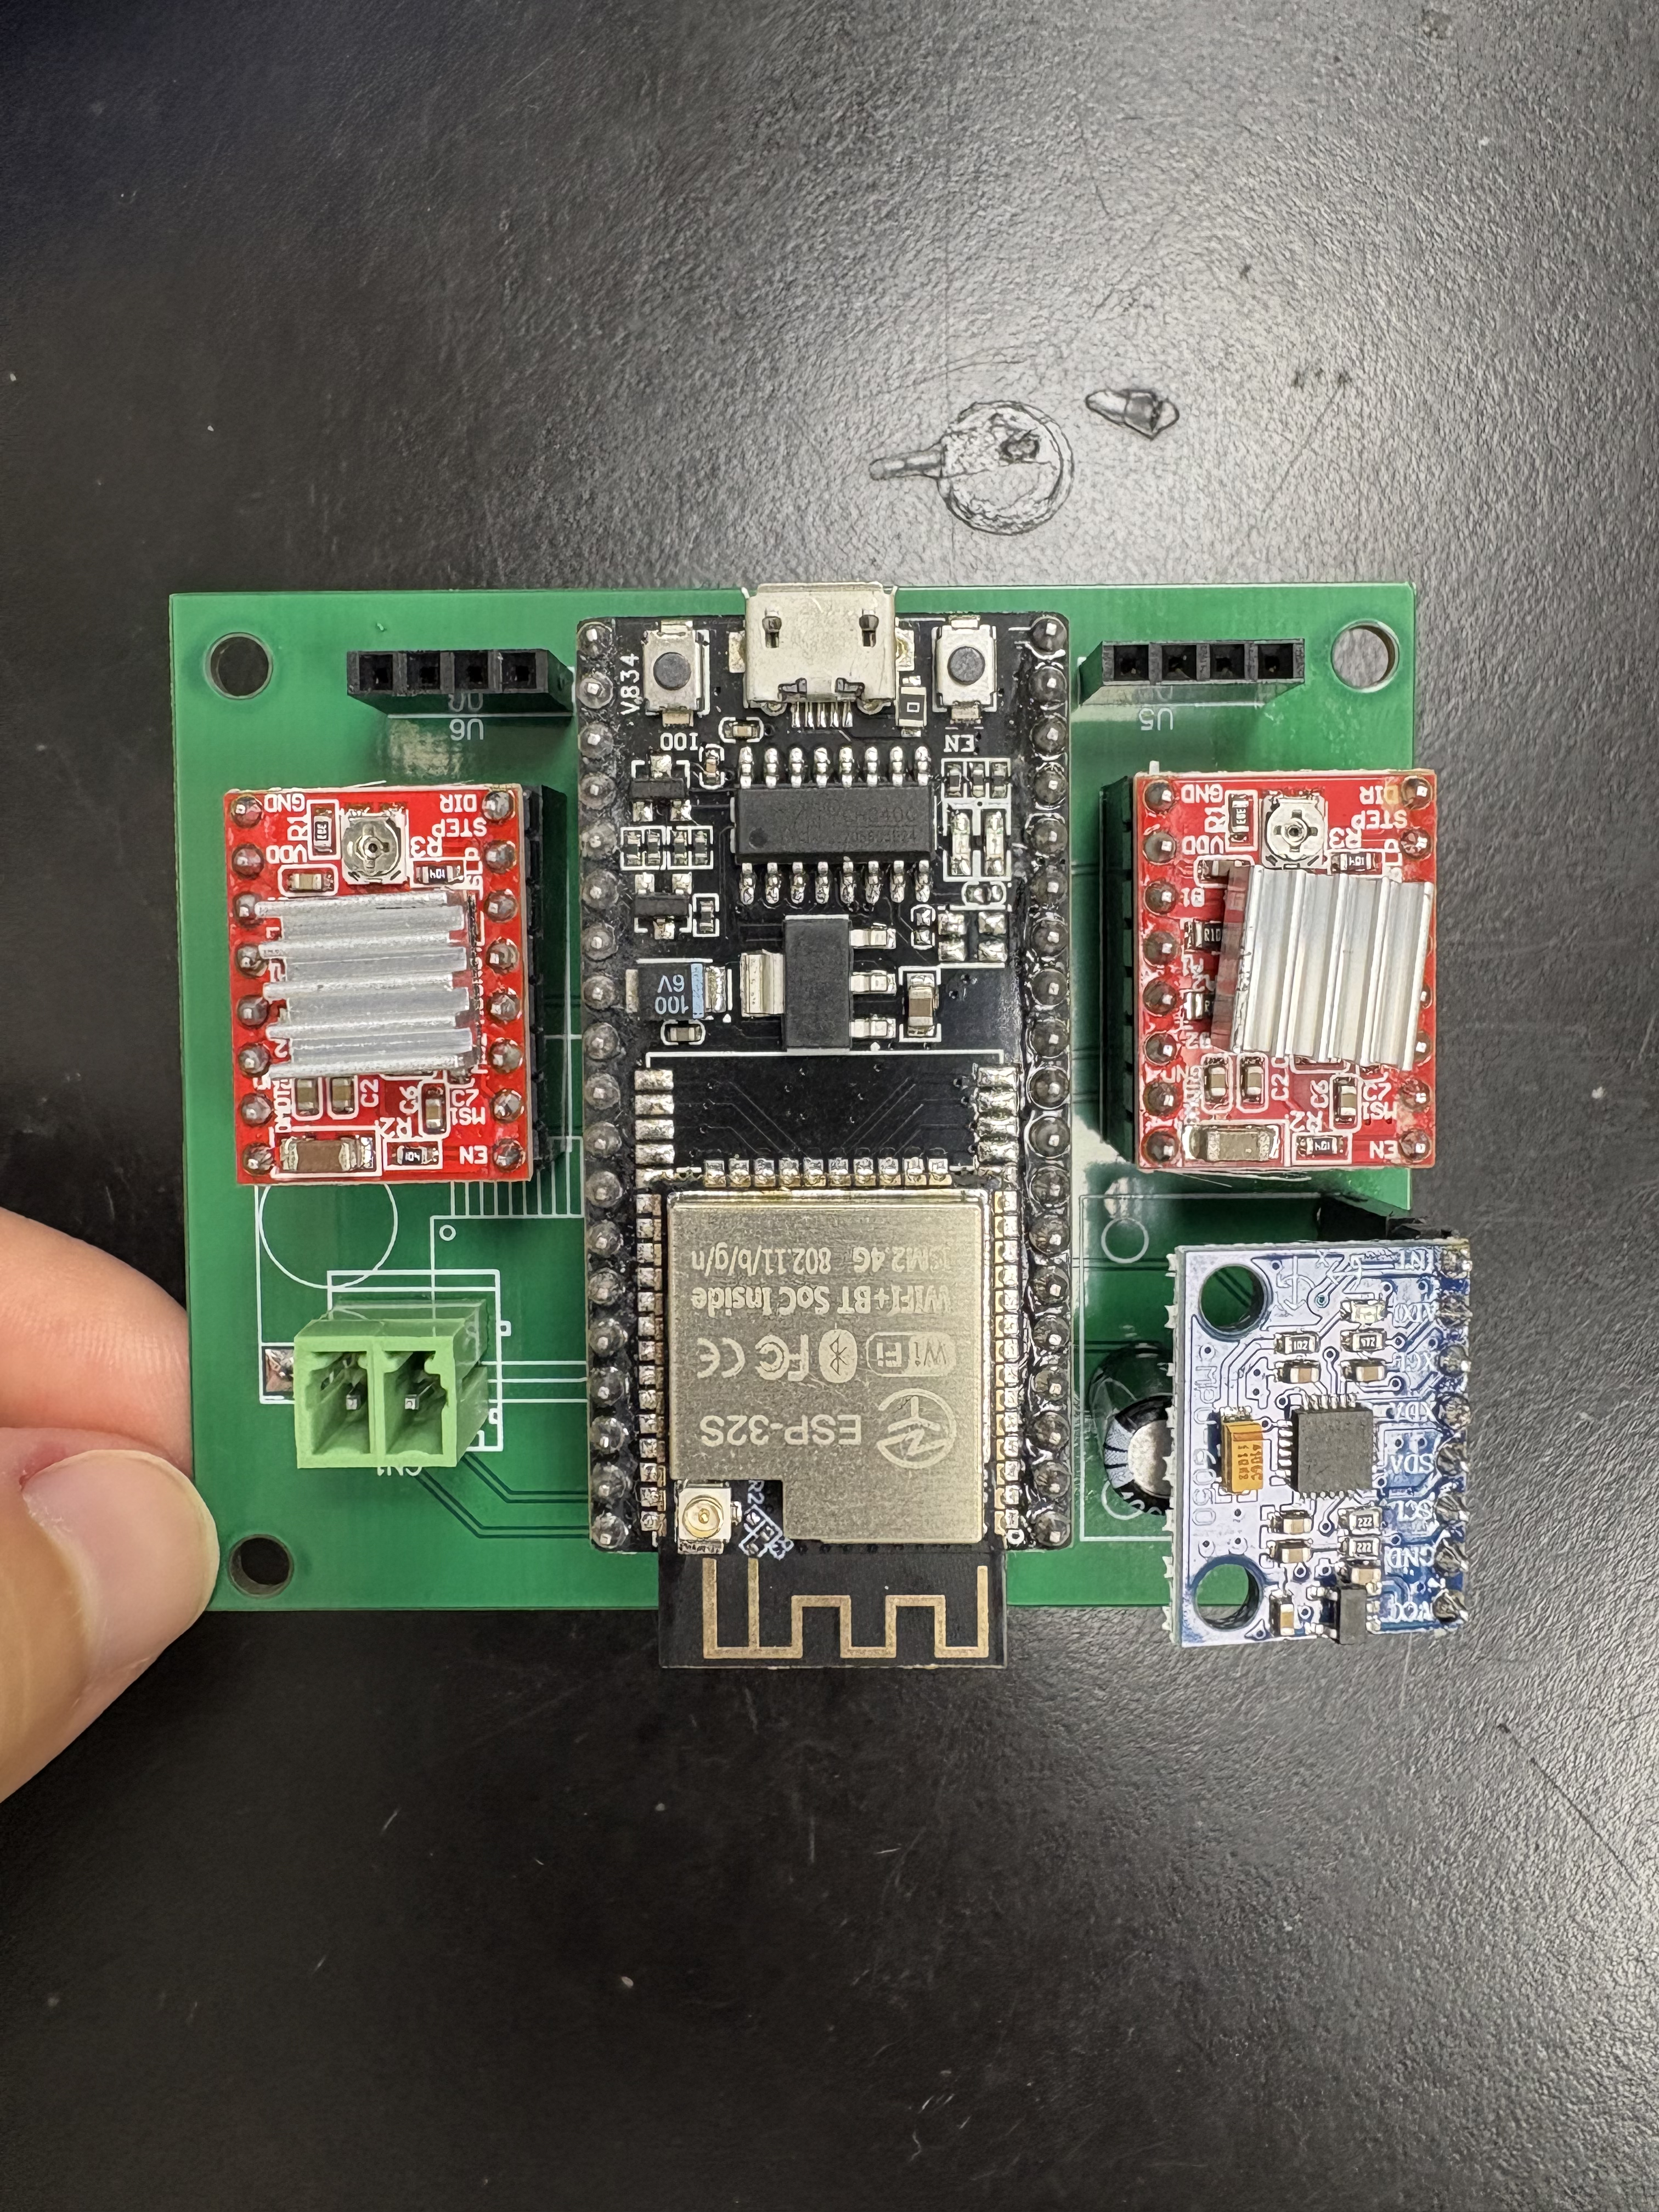
\includegraphics[width=\textwidth]{circuit_photo.png}
        \caption{焊接完成之電路板實作}
        \label{fig:pcb_photo}
    \end{subfigure}
    \caption{平衡車電路邏輯圖與焊接成品}
    \label{fig:pcb_soldered}
\end{figure}

\subsection{Week 10：雷射切割與車體組裝}

\subsubsection{雷射切割}

本組使用 XTool 軟體設計車體木板的切割圖案，並匯入雷射切割機（xTool P2，Class 4 雷射）執行切割，操作全程須確認助教在場。車體設計原則如下：

\begin{itemize}
    \item 黃色標示處為木板相互嵌合的榫接結構（tab-and-slot）。
    \item 紅色標示處為電路板固定孔，需與 PCB 上的螺絲孔位間距對齊。
\end{itemize}

本組設計以企鵝為造型，並在車體側板上刻印「2」作為組別標示，如圖~\ref{fig:laser_design} 所示。雷射切割操作步驟如下：

\begin{enumerate}
    \item 確認助教在場後，打開雷射切割機電源（右後方紅色開關）與抽風機電源。
    \item 以電腦連接雷射切割機，將設計檔案匯入 XTool 軟體並設定切割參數。
    \item 放置木板於切割台，關閉機蓋，按下機器頂部的 Start/Stop 按鈕啟動切割。
    \item 切割過程中留在教室內等待，切割完成後取出木板零件。
\end{enumerate}

\subsubsection{車體組裝}

所需材料：雷射切割完成之木板五片、步進馬達兩個、M3 螺絲十二個、銅柱四個、輪子兩個、聯軸器兩個。組裝步驟如下：

\begin{enumerate}
    \item \textbf{組裝 Side 板與馬達}：將兩塊側板分別與步進馬達組合，注意兩側馬達方向需一致（電線朝同側）。
    \item \textbf{用銅柱固定電路板}：以四個銅柱及 M3 螺絲將 PCB 固定於底板之上，使螺孔位置對齊。
    \item \textbf{組裝主機體}：將底板、側板、中板以榫接結構嵌合，必要時以膠水加固接合處。
    \item \textbf{裝上聯軸器}：將聯軸器接至馬達軸並鎖緊，確保不打滑。
    \item \textbf{裝上輪子}：將輪子套上聯軸器並鎖緊固定螺絲。
    \item \textbf{蓋上上蓋}：將上蓋板嵌入，完成車體。
\end{enumerate}

\subsection{Week 11：ESP32 程式燒錄與 PID 調整}

\subsubsection{開發環境設定}

\begin{enumerate}
    \item 安裝 Arduino IDE 2.0 以上版本，並於 Board Manager 中搜尋「esp32 by Espressif Systems」，安裝版本 \textbf{2.0.7}（注意：高於此版本可能造成不相容問題）。
    \item 將實驗提供之壓縮檔中 \texttt{Library} 資料夾內的模組複製至電腦的 Arduino Library 目錄。
    \item 以文字編輯器開啟 \texttt{defines.h}，將 \texttt{ROBOT\_NAME} 與 \texttt{AP\_PASSWORD} 分別修改為本組的 Wi-Fi 名稱與密碼（本組設定：SSID 為 \texttt{Balancing Robot G2}，密碼為 \texttt{224488861}）。
    \item 於 Arduino IDE 中設定 Board 為「NodeMCU-32S」，Upload Speed 調整為 \textbf{115200}。
    \item 透過 USB 連接 ESP32，上傳程式至開發板。
\end{enumerate}

\subsubsection{PID 參數調整實驗}

\begin{enumerate}
    \item 程式燒錄完成並確認車子能啟動後，以手機連接平衡車建立的 Wi-Fi 熱點（SSID：Balancing Robot G2）。
    \item 以瀏覽器開啟控制介面 \texttt{http://192.168.4.1}，透過介面調整 $K_p$、$K_i$、$K_d$ 數值。
    \item 逐步調整參數，觀察車子平衡狀態，目標是找出至少三組可使系統穩定直立之參數組合。
    \item （延伸）輕推平衡車，觀察車子回復平衡的過程；利用控制介面之 Export CSV 功能匯出感測器時序數據供後續分析。
\end{enumerate}


\section{實驗結果與分析}

\subsection{焊接結果}

本次實驗每位組員各自完成一片 PCB 電路板的焊接。使用有鉛錫線搭配適量焊膏輔助，可讓烙鐵與電路板均勻共熱，使錫線熔化後迅速附著於焊墊，形成光亮的金字塔型銲點。以三用電表導通模式量測各模組插座的 VCC 與 GND 腳位，確認各電源與接地網絡均正常導通，焊接品質達到實驗要求。

\subsection{雷射切割與組裝結果}

本組以企鵝造型設計車體外殼，在側板上刻印「2」作為組別標記，如圖~\ref{fig:laser_result} 所示。

\begin{figure}[H]
    \centering
    \begin{subfigure}[t]{0.45\textwidth}
        \centering
        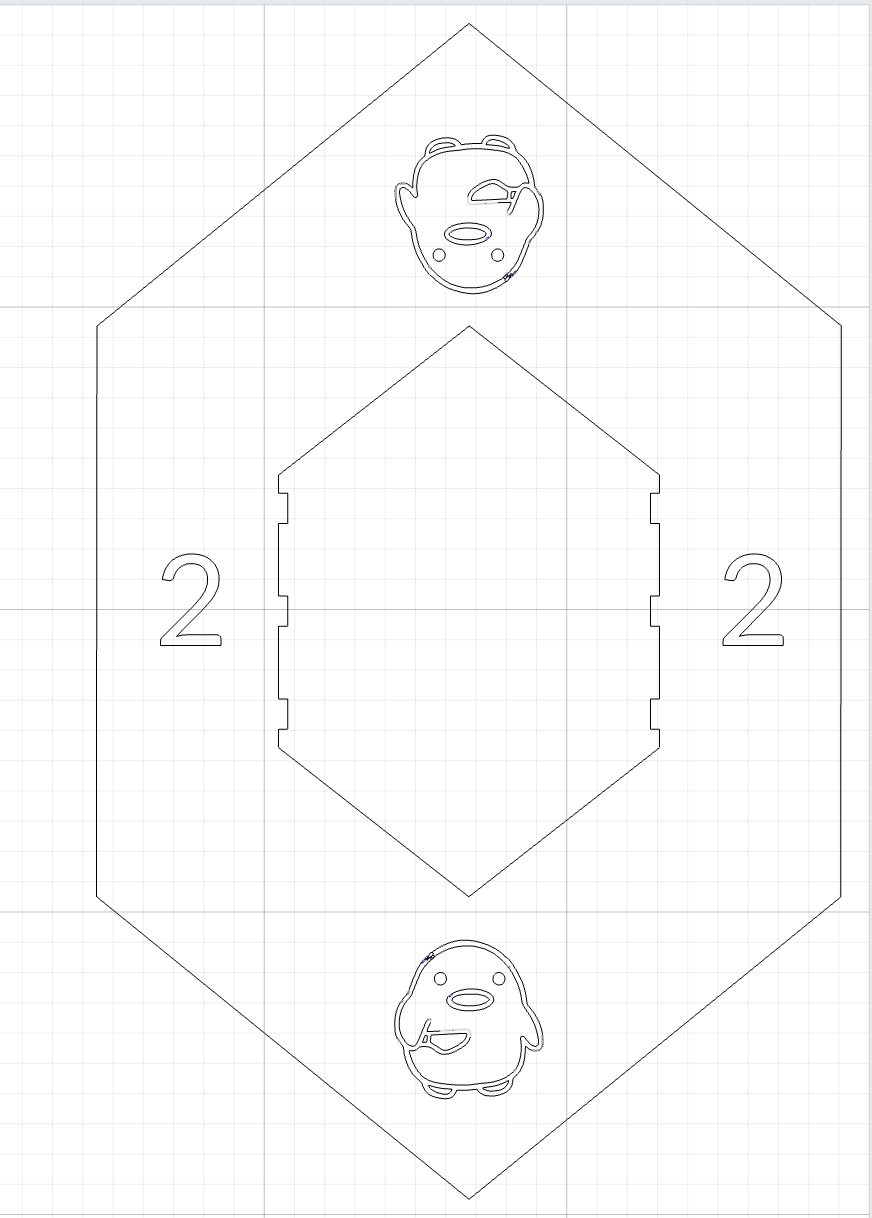
\includegraphics[width=\textwidth]{car_design.png}
        \caption{雷射切割圖設計（企鵝 \& 2）}
        \label{fig:laser_design}
    \end{subfigure}
    \hfill
    \begin{subfigure}[t]{0.45\textwidth}
        \centering
        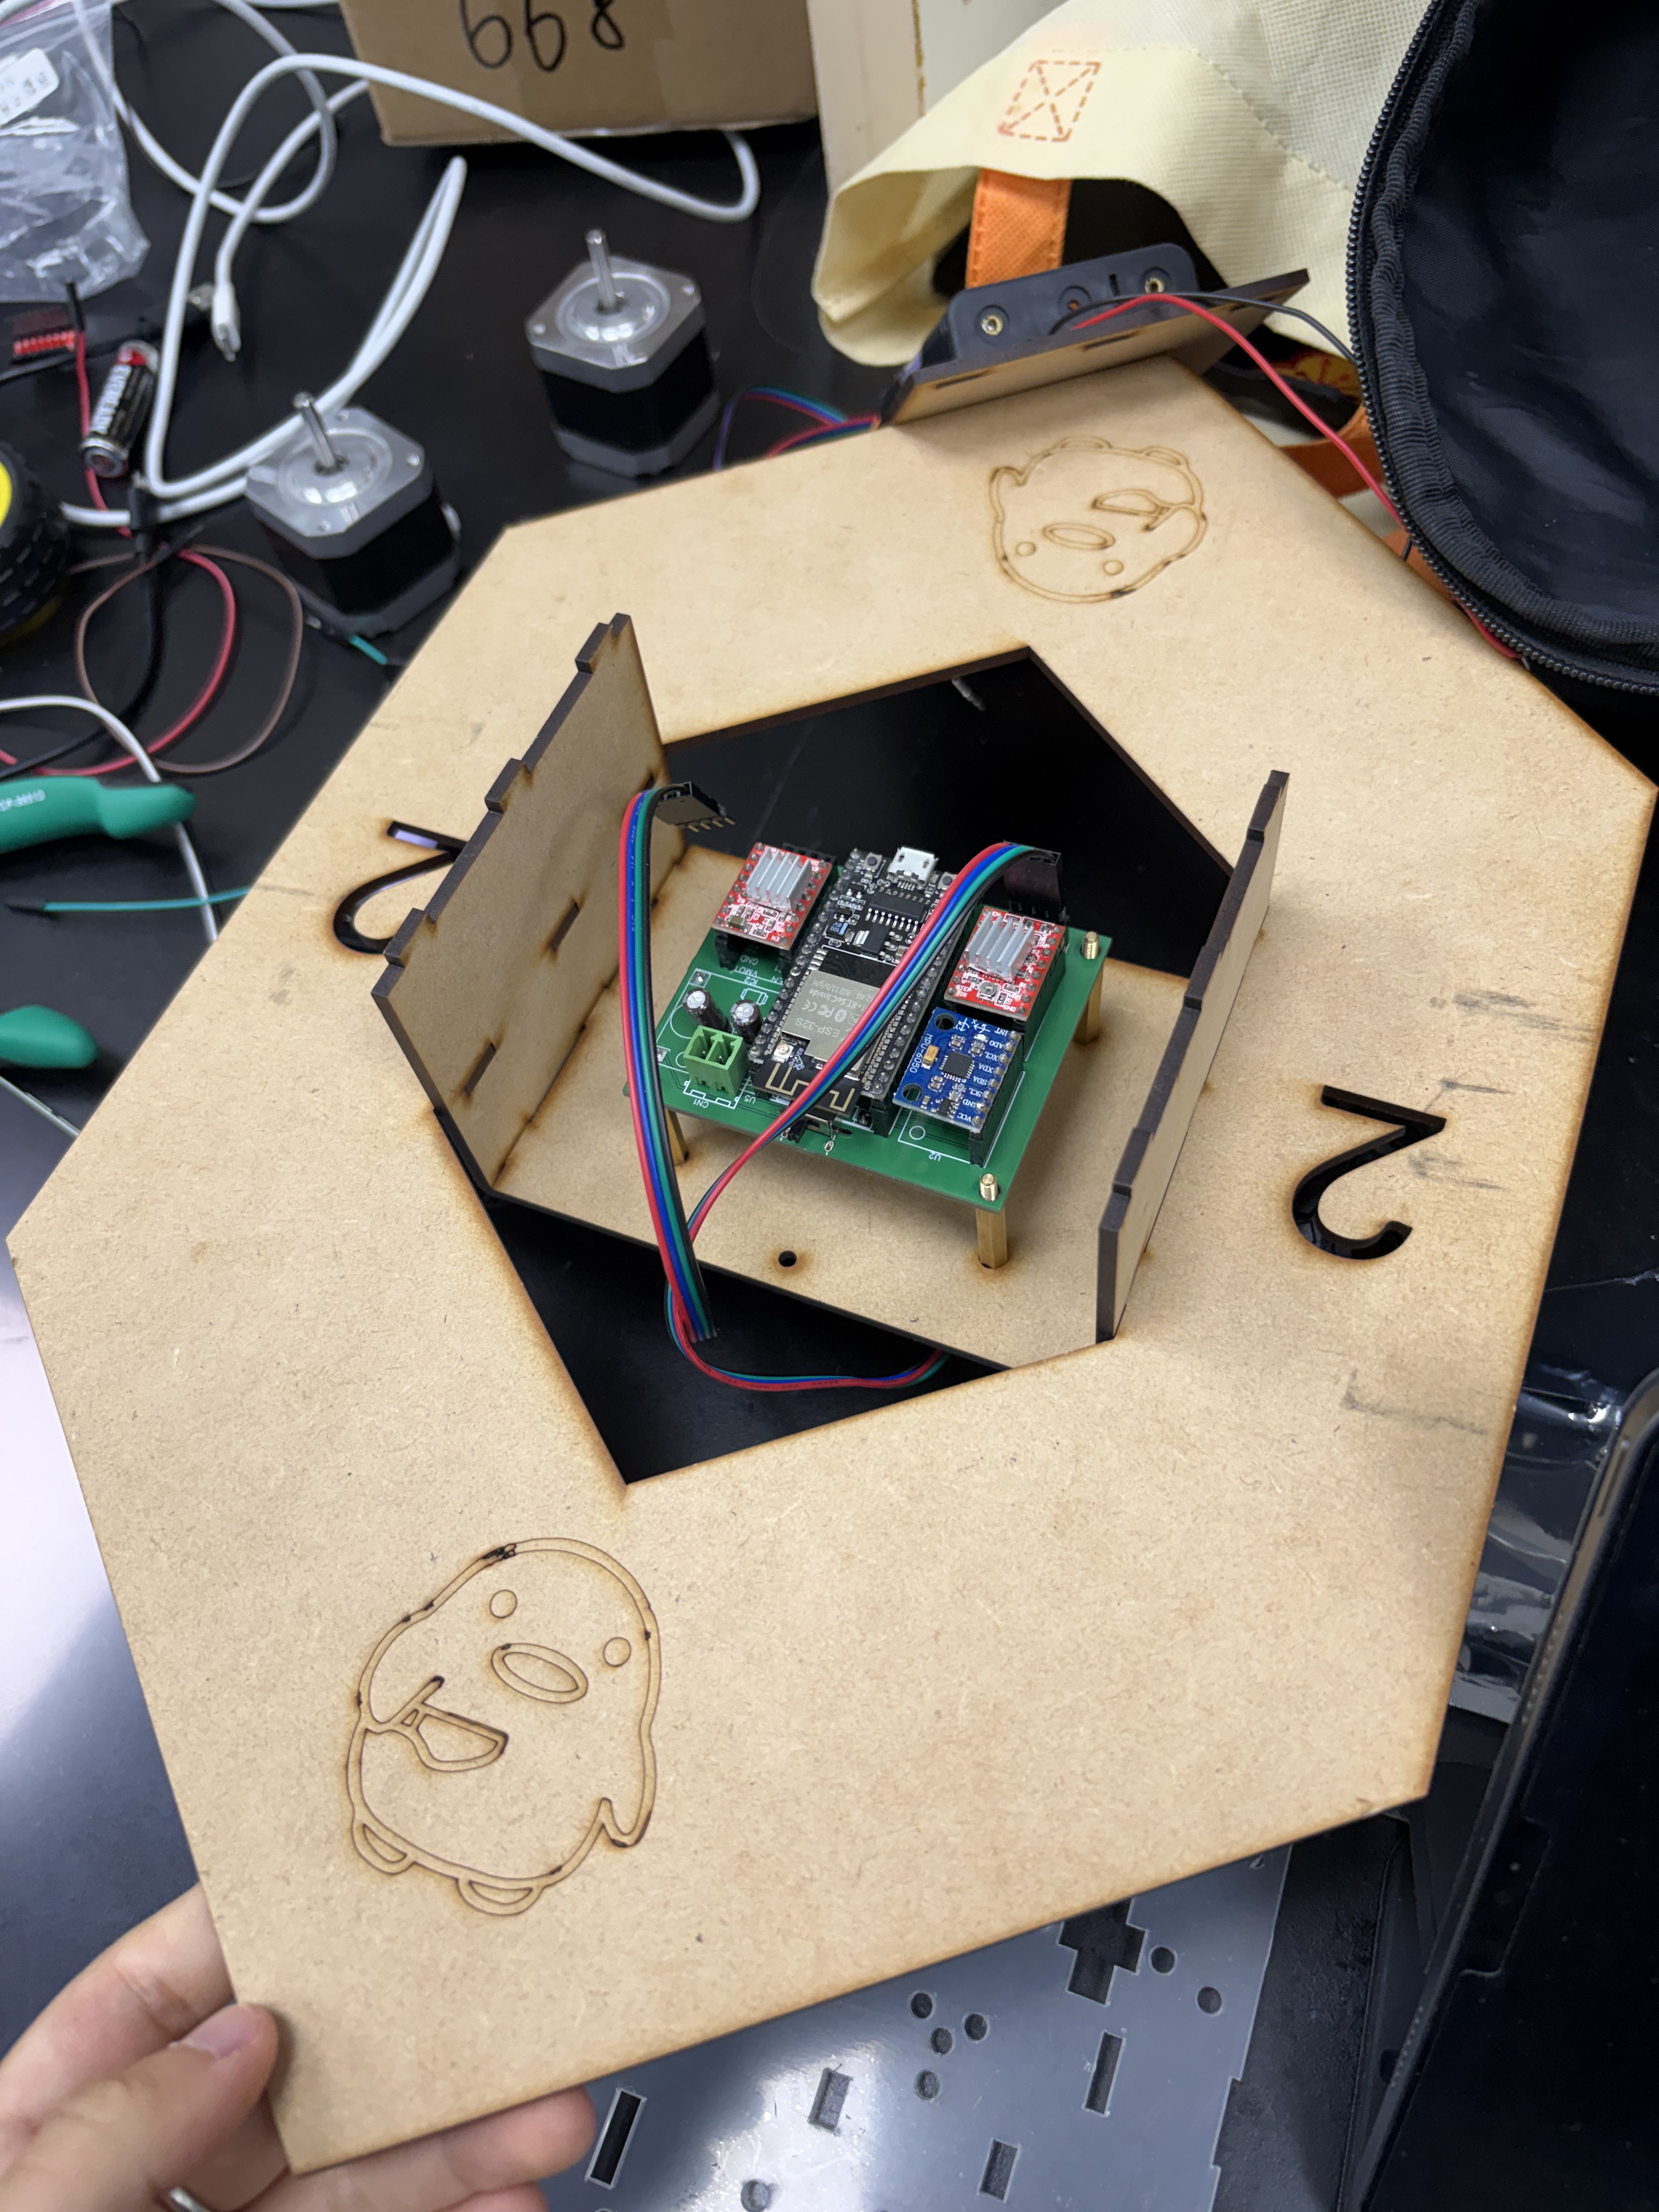
\includegraphics[width=\textwidth]{car.png}
        \caption{組裝完成之平衡車}
        \label{fig:car_assembled}
    \end{subfigure}
    \caption{雷射切割與組裝成果}
    \label{fig:laser_result}
\end{figure}

組裝過程中發現，雷切尺寸與車子本體嵌合時略為過緊。評估後決定將車體本體的寬度縮減約 1\,mm，重新切割後順利完成組裝。此外，考量到原始設計的配重分佈不均，本組在原先設計基礎上加裝後半部車殼，使重心分佈更為均勻，提升平衡穩定性。

\subsection{PID 參數調整結果}

程式燒錄至 ESP32 並啟動平衡車後，透過 Wi-Fi 控制介面調整 PID 參數。初步測試得到一組可使平衡車穩定直立的參數組合，如表~\ref{tab:pid_result} 所示。

\begin{table}[H]
    \centering
    \begin{tabular}{ccc}
        \hline
        $K_p$ & $K_i$ & $K_d$ \\
        \hline
        2.2 & 0.29 & 0.289 \\
        \hline
    \end{tabular}
    \caption{本組初步測試可使平衡車穩定直立之 PID 參數}
    \label{tab:pid_result}
\end{table}

在此參數組合下，平衡車可在平地上持續直立並自主移動。調整 $K_d$ 值的效果最為直觀：當 $K_d = 0$ 時，車子會劇烈前後搖晃（overshoot / oscillation）；隨著 $K_d$ 逐漸增大，震盪幅度明顯收斂，與表~\ref{tab:pid_effects} 中的理論預測吻合。

\subsection{問題排查：左輪異常}

完成初步 PID 測試後不久，車子出現左輪間歇性不轉動的問題，導致無法繼續測試更多 PID 組合。本組對此進行了以下系統性排查：

\begin{enumerate}
    \item \textbf{更換左側馬達}：排除馬達本身損壞的可能性，問題仍然存在。
    \item \textbf{更換馬達驅動模組（A4988）}：排除驅動 IC 損壞的可能性，問題仍然存在。
    \item \textbf{重新焊接 A4988 模組腳位}：確認焊點無虛焊後，問題仍然存在。
\end{enumerate}

經助教以三用電表量測後，發現左側 A4988 模組的輸出端電壓異常偏低，推測問題可能出在 PCB 走線或焊接端存在較高的接觸電阻，但確切原因仍待進一步追查。由此可見，在多模組整合的電路系統中，故障排除需系統性地逐一排除各子系統，並善用電表量測各節點電位，才能有效縮小問題範圍。


\section{問題討論}


\subsection{請寫下焊接和雷射切割作業可能遭遇的危險，以及預防方式各兩點。}

\subsection{在實驗⼀中，在沒有D的狀態下，⾞⼦會劇烈的前後搖晃。這是前⾯所說的Overshoot/Oscillation 問題，在D提升⾄特定值後會有所改善。請問若忽略I，給定特定的P，能讓系統最穩定的D和P的關係為何？可以⽤實驗⼀取得的數據畫趨勢圖分析，也可以解前⾯的微分⽅程式，或⽤軟體分析結果}

\subsection{當PID 參數沒有最佳化時，平衡⾞容易因為些微的噪⾳被放⼤⽽失衡。除了直接更改PID 參數外，有什麼
⽅法可以減少噪⾳的影響？ 可以就控制程式，硬體或⾞體設計討論}


\end{document}